\subsection{MetaPCA}
Dimension reduction is a popular data mining approach for transcriptomic analysis.
MetaPCA aims to combine multiple omics datasets of identical or similar biological hypothesis and perform simultaneous dimensional reduction in all studies.
The results show improved accuracy, robustness and better interpretation among all studies.
By clicking toolsets and then metaPCA,
users are directed to metaPCA home page as Figure~\ref{fig:metaPCAHome}.
The R package for MetaPCA module can be found \url{https://github.com/metaOmics/metaPCA}.

\begin{figure}[H]
\begin{center}
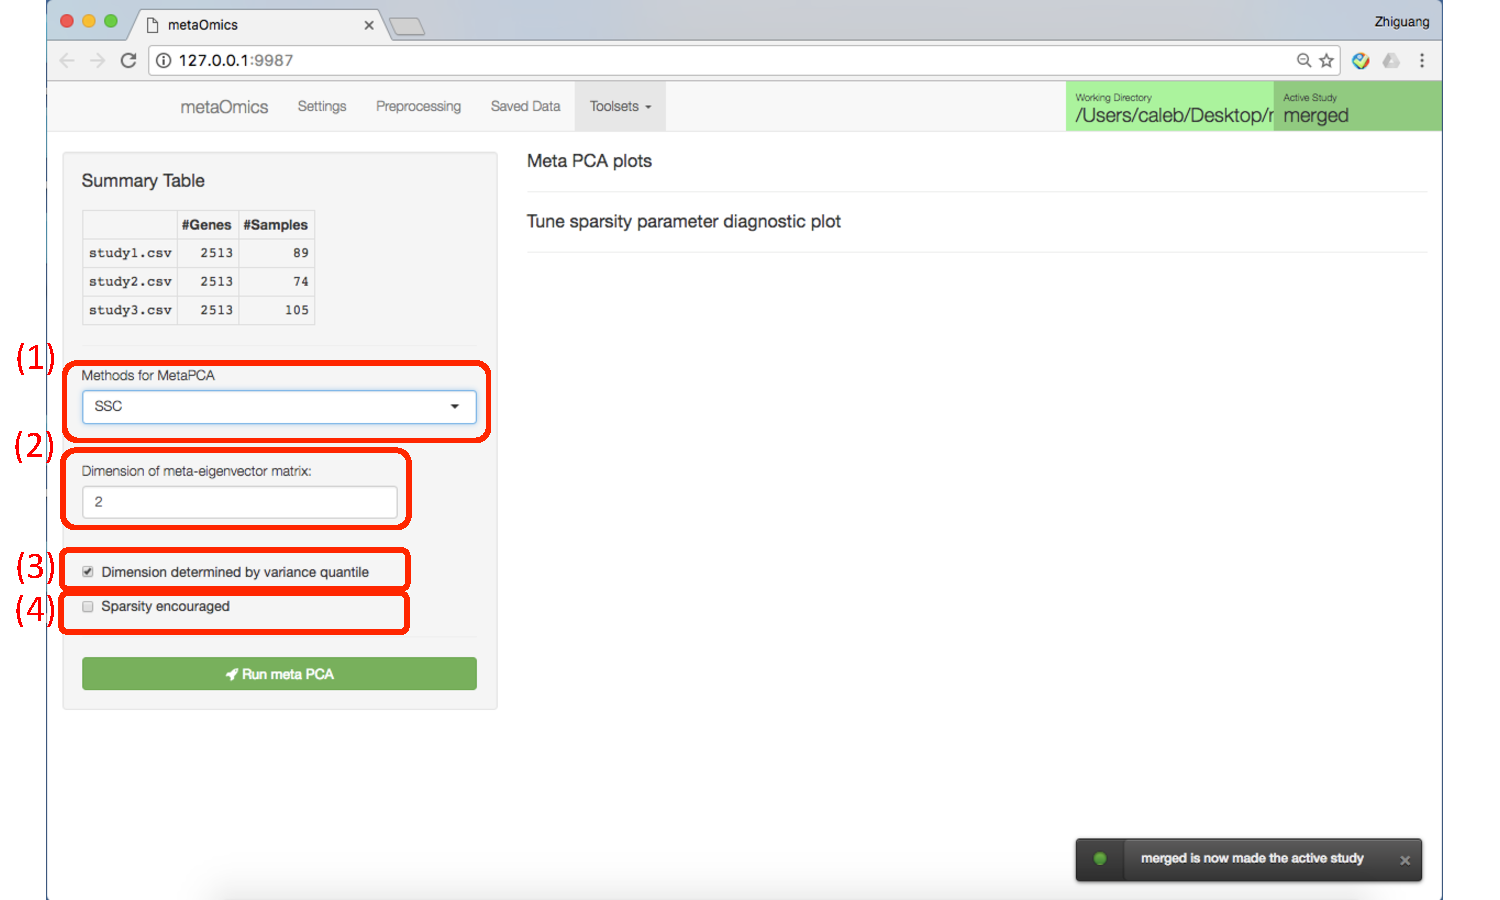
\includegraphics[scale=0.4]{./figure/metaPCA/metaPCAHome.pdf}
\caption{MetaPCA settings}
\label{fig:metaPCAHome}
\end{center}
\end{figure}

\subsubsection{Procedure}

\begin{steps}

\item \textbf{Specify parameters} 

There are very few parameter to be specify in metaPCA, as in Figure~\ref{fig:metaPCAHome}.
Advanced options are not suggested to change unless the users are familiar with the algorithm.
There are two methods for MetaPCA (at position {\color{red} (1)}). 
SSC represent MetaPCA via sum of squared cosine (SSC) maximization.
SV represent MetaPCA via sum of variance decomposition (SV).
Details of SSC and SV can be found in metaPCA manuscript.
SSC has better performance and is suggested.
Dimension of meta-eigenvector matrix option (at position {\color{red} (2)}) allows user to specify dimension of the output meta-eigenvector matrix.
The checkbox of ``dimension determined by variance quantile" is suggested to be selected (at position {\color{red} (3)}).
If it is selected, the dimension size of each study's eigenvector matrix (SSC) is determined  by the pre-defined level of variance quantile 80\%.
If the checkbox of ``sparsity encouraged" is selected (at position {\color{red} (4)}), users can perform metaPCA.
After clicking on search for optimal tuning parameter button, the optimum tuning parameter will be returned to the box ``tuning parameter for sparsity", 
which may be time consuming.

\item \textbf{Perform metaPCA} 

By clicking the ``Run meta PCA" button, MetaPCA will be performed.


\end{steps}

\textbf{Complete List of Options:} 
\begin{enumerate}
\item Common metaPCA parameters: 

\begin{itemize}
\item Methods for metaPCA:
SSC represent MetaPCA via sum of squared cosine (SSC) maximization.
SV represent MetaPCA via sum of variance decomposition (SV).
\item Dimension of meta-eigenvector matrix: dimension of the output meta-eigenvector matrix.
\item Dimension determined by variance quantile:
the dimension size of each study's eigenvector matrix (SSC) is determined  by the pre-defined level of variance quantile 80\%.
\end{itemize}

\item If sparsity encouraged is selected, there are extra tuning parameter ($\lambda$) that may need to be tuned.

\begin{itemize}
\item  Min $\lambda$: lower bound of the searching space of $\lambda$.
\item Max $\lambda$: upper bound of the searching space of $\lambda$.
\item Step of of $\lambda$: stepsize of the searching space of $\lambda$.
\item Tuning parameter for sparsity: Tuning parameter for sparsity that will be used for sparse metaPCA.
\end{itemize}


\end{enumerate}


\subsubsection{Results}
The input dataset is same as the input for MetaDE module.
We used multi-study leukemia gene expression data as example.
After performing merging of the three datasets and filter 50\% genes by mean and 50\% by variance, 1283 genes remained.
Detailed descriptions of these studies can be found in Table~\ref{tab:realDataLeukemia}. 

The result of metaPCA is shown in Figure~\ref{fig:metaPCAresult}.
For each study, only first two studies are visualized.
The results show nice separations between three groups.
These figures and eigenvectors from metaPCA are saved.

\begin{figure}[H]
\begin{center}
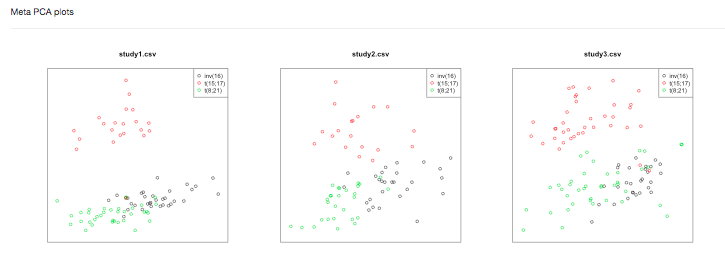
\includegraphics[scale=0.3]{./figure/metaPCA/metaPCA}
\caption{MetaPCA result}
\label{fig:metaPCAresult}
\end{center}
\end{figure}

